\documentclass[11pt]{article}

\usepackage{times}
\usepackage{alltt}
\usepackage{hyperref}
\usepackage{graphicx}
%% Generic environments and commands that we use in the CS:APP book

%%%%%%%%%% 
% Commands
%%%%%%%%%% 

% For putting labels on pictures
\newcommand{\clabel}[1]{\makebox(0,0){#1}}
\newcommand{\rlabel}[1]{\makebox(0,0)[r]{#1}}
\newcommand{\llabel}[1]{\makebox(0,0)[l]{#1}}
\newcommand{\blabel}[1]{\makebox(0,0)[b]{#1}}
\newcommand{\lblabel}[1]{\makebox(0,0)[lb]{#1}}
\newcommand{\tlabel}[1]{\makebox(0,0)[t]{#1}}

%% Comment command
\newcommand{\comment}[1]{}

%% Two part captions.  First part is title.  Second is explanation.
\newcommand{\mycaption}[2]{\caption[#1]{{\bf #1} #2}}

%%%%%%%%%%%%%%%%%%%%%%%%%%%%%%%%%%%%%%%%%%%%%%%%%%%%%%%%%%%% 
% Environments and macros for different elements of the book
%%%%%%%%%%%%%%%%%%%%%%%%%%%%%%%%%%%%%%%%%%%%%%%%%%%%%%%%%%%%% 

%% Various Unix command-line prompts
\newcommand{\unixprompt}{unix>}
\newcommand{\linuxprompt}{linux>}
\newcommand{\solarisprompt}{solaris>}

%% pcode- Generating pseudo-code
\newenvironment{pcode}{\mbox{}\newline\vspace{.5ex}\newline\begin{minipage}{6in}\begin{tt}\begin{tabbing}MM\=MM\=MM\=MM\=MM\=MM\=MM\=MM\=MM\=\+\kill}{\end{tabbing}\end{tt}\end{minipage}\newline\vspace{.5ex}\newline}

%% Showing syntactic elements in pseudo-code
\newcommand{\syntax}[1]{{\rm\it #1}}

%% aside - for displaying sidebars 
\newenvironment{aside}[1]%
{\begin{quote}\footnotesize{\bf Aside: #1\\}}
{{\bf End Aside.}\end{quote}}

%% ntc - New to C element
\newenvironment{ntc}%
{\begin{quote}\footnotesize{\bf New to C?}\\}
{{\bf End}\end{quote}}

%% ccode- for displaying formatted C code (c2tex) 
\newenvironment{ccode}%
{\small}%
{}

%% scode - for displaying formatted ASM code (s2tex and d2tex)
\newenvironment{scode}%
{\small}
{}

%% codefrag - for displaying unformatted code fragments
\newenvironment{codefrag}%
{\small\begin{alltt}}%
{\end{alltt}%
}

%% tty - for displaying TTY input and output
\newenvironment{tty}%
{\small\begin{alltt}}%
{\end{alltt}}


%% Environment for descriptions that provide aligned text
\newenvironment{mydesc}[1]{
\setbox1=\hbox{#1}
\begin{list}{}{
\setlength{\labelwidth}{\wd1}
\setlength{\leftmargin}{\wd1}
  \addtolength{\leftmargin}{1em}
  \addtolength{\leftmargin}{\labelsep}
\setlength{\rightmargin}{1em}}}{\end{list}}

\newcommand{\litem}[1]{\item[#1\hfill]}
\newcommand{\ritem}[1]{\item[#1]}

%%%%%%%%%%%%%%%%%%%%%%%%%%%%%%%%%%%%%%%%%%%%%%%%%%%%%%%%%%%%%%%%%%%%%%%%%%%%
%% Indexing 
%%%%%%%%%%%%%%%%%%%%%%%%%%%%%%%%%%%%%%%%%%%%%%%%%%%%%%%%%%%%%%%%%%%%%%%%%%%%
%% Distinguish 5 types of index entries
%%   - IA32 instructions (iindex, diindex)
%%   - Program names (pindex, dpindex)
%%   - C things (cindex, dcindex)
%%   - Stdlib functions (sindex, dsindex)
%%   - Unix functions (uindex, duindex)
%%   - CSAPP functions (csindex, dcsindex)
%%   - CSAPP programs (pcsindex, dpcsindex)
%%   - Library files, such as <limits.h> (lindex, dlindex) 
%%   - Everything else. (index, dindex)
%% In every case, the `d' version is used for the definining index entry

%% IA32 instructions.
%% Takes two arguments:
%% The name of the instruction
%% An English rendition of the mnemonic
\newcommand{\iindex}[2]{\index{#1@{\tt #1} [IA32] #2}}
\newcommand{\diindex}[2]{\index{#1@{\tt #1} [IA32] #2|emph}}

%% Program names (e.g., gcc, gdb.  Write in lower case)
%% Takes two arguments:
%% The name of the program
%% An English description
\newcommand{\pindex}[2]{\index{#1@{\sc #1} #2}}
\newcommand{\dpindex}[2]{\index{#1@{\sc #1} #2|emph}}

%% C things (operators, statements, etc)
%% Takes two arguments:
%% C name
%% An English description
\newcommand{\cindex}[2]{\index{#1@{\tt #1} [C] #2}}
\newcommand{\dcindex}[2]{\index{#1@{\tt #1} [C] #2|emph}}

%% Stdlib functions
%% Takes two arguments:
%% function name
%% An English description
\newcommand{\sindex}[2]{\index{#1@{\tt #1} [C Stdlib] #2}}
\newcommand{\dsindex}[2]{\index{#1@{\tt #1} [C Stdlib] #2|emph}}

%% Unix functions
%% Takes two arguments:
%% function name
%% An English description
\newcommand{\uindex}[2]{\index{#1@{\tt #1} [Unix] #2}}
\newcommand{\duindex}[2]{\index{#1@{\tt #1} [Unix] #2|emph}}

%% CSAPP functions
%% Takes two arguments:
%% function name
%% An English description
\newcommand{\csindex}[2]{\index{#1@{\tt #1} [CS:APP] #2}}
\newcommand{\dcsindex}[2]{\index{#1@{\tt #1} [CS:APP] #2|emph}}

%% CSAPP programs
%% Takes two arguments:
%% function name
%% An English description
\newcommand{\pcsindex}[2]{\index{#1@{\sc #1} [CS:APP] #2}}
\newcommand{\dpcsindex}[2]{\index{#1@{\sc #1} [CS:APP] #2|emph}}

%% Library file names (e.g., <limits.h>)
%% Takes two arguments:
%% The name of the file (without brackets)
%% An English description
\newcommand{\lindex}[2]{\index{#1@{\tt <#1>} #2}}
\newcommand{\dlindex}[2]{\index{#1@{\tt <#1>} #2|emph}}

%% Normal index entry.
%% Takes one argument
%% \index already defined
\newcommand{\dindex}[1]{\index{#1|emph}}


%% Page layout
\oddsidemargin 0pt
\evensidemargin 0pt
\textheight 600pt
\textwidth 469pt
\setlength{\parindent}{0em}
\setlength{\parskip}{1ex}

\begin{document}

\title{CSCI340, Fall 2014\\
Assignment 5: Writing a Scheduler
}

\author{California State University - Chico\\
  By Bryan Dixon\\
}
\date{\emph{Due Date: Sunday, April 12th, 2015 11:59pm}}


\maketitle

\section*{Introduction}
The purpose of this assignment is for you gain insight into how schedulers work on the system. 

\section*{Logistics}

The only ``hand-in'' will be
electronic.  Any clarifications and revisions to the assignment will
be posted on my web page and emailed out to the class.

\section*{Hand Out Instructions}

I recommend you use an Ubuntu Linux virtual machine to complete this
assignment.  Alternatively, you can use the jaguar machines or your native Linux install. 

Download the file \texttt{scheduler-handout.tar} from the course
``assignment'' page.

Start by copying the file {\tt scheduler-handout.tar}
to the protected directory (the {\em lab directory}) in which you plan
to do your work.  Then do the following:

\begin{itemize}
\item Type the command {\tt tar xvf scheduler-handout.tar} 
to expand the tarfile.

\item Type the command {\tt make} to compile and link some
test routines.

\item Enter your name in the header
comment at the top of {\tt schedule.cc}.

\end{itemize}

Looking at the {\tt schedule.cc} file, you will see that it contains a rudimentary scheduler API to add a process, remove a process, and get the next process from your scheduler. Your job is to implement the code in schedule.cc that implements a variant of a Multi Level Priority Scheduler using Round Robin schedulers. 

\begin{figure}[htbp]
  \begin{center}
    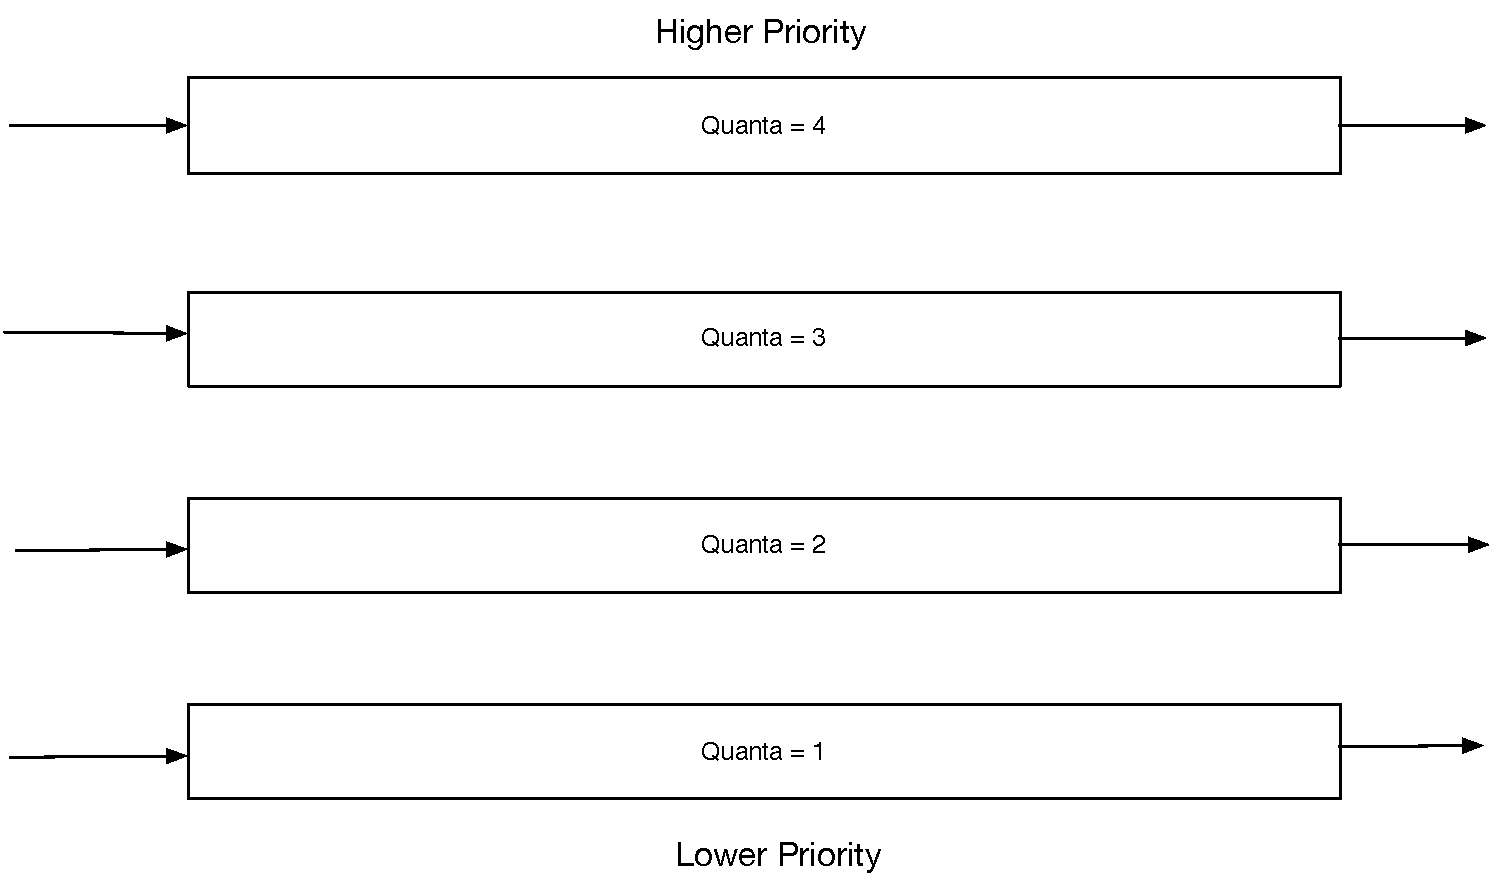
\includegraphics[width=150mm]{multilevel.pdf}
    \caption{Multi Level Round Robin Priority Scheduler}
    \label{fig:multilevel}
  \end{center}
\end{figure}

\section*{General Overview of Schedulers}
\emph{Taken from Wikipedia\cite{schedules}}

In computer science, scheduling is the method by which threads, processes or data flows are given access to system resources (e.g. processor time, communications bandwidth). This is usually done to load balance and share system resources effectively or achieve a target quality of service. The need for a scheduling algorithm arises from the requirement for most modern systems to perform multitasking (executing more than one process at a time) and multiplexing (transmit multiple data streams simultaneously across a single physical channel).

The scheduler is concerned mainly with:

\begin{itemize}
\item \textbf{Throughput} - The total number of processes that complete their execution per time unit.
\item \textbf{Latency}, specifically:
\begin{itemize}
        \item \textbf{Turnaround time} - total time between submission of a process and its completion.
        \item \textbf{Response time} - amount of time it takes from when a request was submitted until the first response is produced.
\end{itemize}
\item \textbf{Fairness} - Equal CPU time to each process (or more generally appropriate times according to each process' priority and workload).
\item \textbf{Waiting Time} - The time the process remains in the ready queue.
\end{itemize}

In practice, these goals often conflict (e.g. throughput versus latency), thus a scheduler will implement a suitable compromise. Preference is given to any one of the above mentioned concerns depending upon the user's needs and objectives.

In real-time environments, such as embedded systems for automatic control in industry (for example robotics), the scheduler also must ensure that processes can meet deadlines; this is crucial for keeping the system stable. Scheduled tasks can also be distributed to remote devices across a network and managed through an administrative back end.

\section*{Your Task}

The task for this assignment is to implement the scheduler API provided to you in the {\tt schedule.cc} file with variant of a multi level priority scheduler using Round Robin schedulers. This scheduler iterates through the different levels starting with the highest priority (priority 1) and choses the process next in the queue for that priority level to schedule for a specified quanta or time. The higher the priority the more quanta is given. Your implementation should mirror the quanta and number of priorities shown in Figure \ref{fig:multilevel}. 

You aren't allowed to import any libraries not already provided in the {\tt schedule.cc} file.

\section*{Data Structures in C}
As you can't include any libraries for data structures you'll likely want to implement your own data structure to implement the FCFS scheduler. As such you'll need to do this in C code. As an example here is a simple implementation of a linked list in C using structs:

\begin{verbatim}
#include <stdio.h>
#include <stdlib.h>

struct node {
    int value;
    struct node *next;
};

int main(){
    int i;
    /* This will be the unchanging first node */
    struct node *root;
    /* cur node for manipulating linked list */
    struct node *cur;      

    /* 
    * Now root points to a node struct 
    * Dynamic allocation of memory the size of 
    * a node in C (similar to new node in C++)
    */
    root = (struct node *) malloc( sizeof(struct node));

    cur = root;
    for(i=0; i<10;i++){
        cur->value = i;
        cur->next = (struct node *) malloc( sizeof(struct node));
        cur = cur->next;
    }
    //Create final values
    cur->value = 10;
    cur->next = NULL;

    /* Now let's print it out */
    cur=root;
    while(cur){
        printf("%d ", cur->value);
        cur=cur->next;
    }
    printf("\n");

    /* Let's free up memory */
    while(root){
        cur = root;
        root = root->next;
        free(cur); //like delete
    }          
}
\end{verbatim}



\section*{Checking Your Work}

I have provided some tools to help you check your work.

{\bf Reference solution.} I've included a reference output file with the expected solution. Your program should produce identical output to that of the {\tt ref.out} file. There is also a {\tt simref} executable that will generate the reference output as well. 

\section*{Hints}

\begin{itemize}
\item Read {\bf Section 6.3} of the Operating System Concepts Essentials 2nd edition
book. 


\end{itemize}

\section*{Evaluation}

Your solution will be tested agains the reference output. You will get full credit if your assignment reproduces the reference output. 

\section*{Hand In Instructions}

You only have to change {\tt schedule.cc}.  You need to upload
 {\tt schedule.cc} to the \url{http://turnin.ecst.csuchico.edu/} page to mark your completion
time.

\section*{Extra Credit - 10pts}

I'm in the process of working out a potential EC scheduler for you to implement in addition to this assignment. If one gets created details will be updated here. 

\begin{thebibliography}{3}

\bibitem{schedules} Wikipedia.
  \newblock ``Scheduling (computing)''.
  \newblock Wikipedia, The Free Encyclopedia. 2012.
  \newblock
  \url{http://en.wikipedia.org/wiki/Process_scheduler}.
  \newblock Online; accessed 16-February-2014.

\end{thebibliography}
\end{document}
